\documentclass{beamer}

\mode<presentation>{
\usetheme{Madrid}
\setbeamertemplate{navigation symbols}{}
}

\usepackage{graphicx}
\usepackage{booktabs}
\usepackage[spanish]{babel}
\usepackage[latin1]{inputenc}

%====================================

\title[Trabajo de fin de m�ster]{Redes Generativas Antag�nicas}

\author[Ant�n Makarov]{Ant�n Makarov Samusev}
\institute[UCM/UPM]
{
Universidad Complutense de Madrid \\
\medskip
Universidad Polit�cnica de Madrid \\
\medskip
\textit{amakarov@ucm.es}
}
\date{25 de septiembre de 2019}

%====================================

\begin{document}

\begin{frame}
\titlepage
\end{frame}

%------------------------------------------------

\begin{frame}
\frametitle{�ndice}
\tableofcontents
\end{frame}

%------------------------------------------------

%====================================
%Para incluir graficas
%\begin{figure}
%\includegraphics[width=0.8\linewidth]{test}
%\end{figure}
%====================================

%------------------------------------------------
\section{Redes Generativas Antag�nicas}
%------------------------------------------------

\begin{frame}
	\frametitle{Objetivo}
	
\end{frame}

\begin{frame}
\frametitle{Idea conceptual}
\begin{figure}
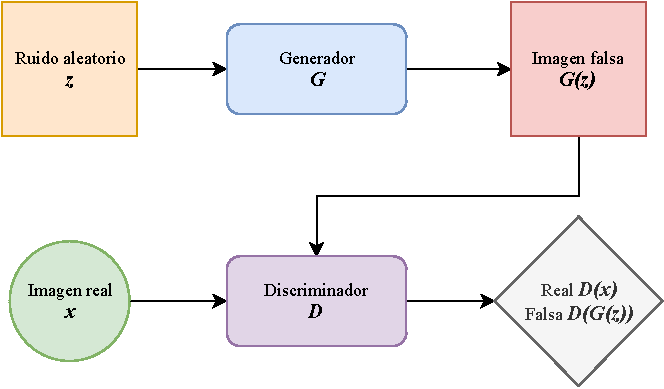
\includegraphics[width=0.8\linewidth]{../images/report/scheme.pdf}
\end{figure}
\end{frame}

\begin{frame}
\frametitle{Aspectos te�ricos}
\begin{equation*}
\min_G \max_D V(G,D) = \mathbb{E}_{x \sim p_d(x)} [\log D(x)] + \mathbb{E}_{z \sim p_z(z)} [\log (1- D(G(z)))].
\label{minimax}
\end{equation*}
\end{frame}

%------------------------------------------------
\section{Generaci�n de arte}
\subsection{DCGAN}
%------------------------------------------------

\begin{frame}
\frametitle{DCGAN}

\end{frame}

%------------------------------------------------
\subsection{Metodolog�a}
%------------------------------------------------

\begin{frame}
	\frametitle{Obtenci�n y pre-procesado}
	
\end{frame}

\begin{frame}
\begin{figure}
	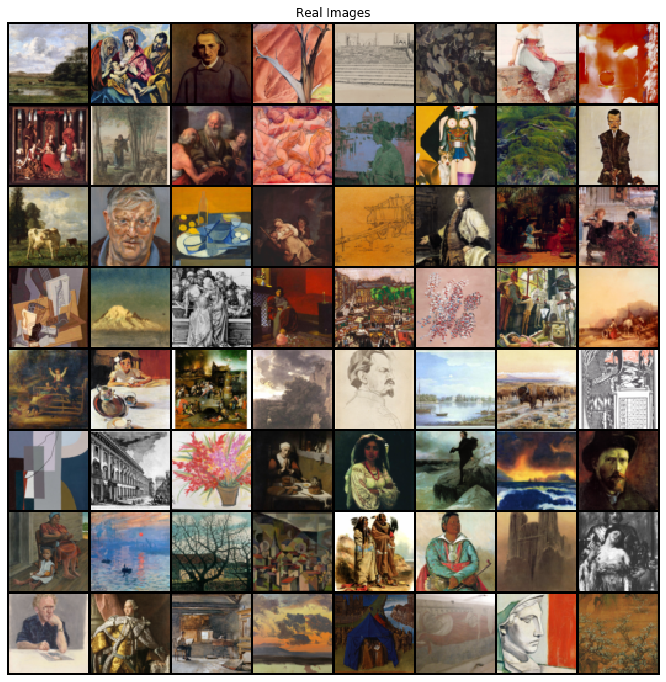
\includegraphics[width=0.7\linewidth]{../images/results/original_data.png}
\end{figure}
\end{frame}

\begin{frame}
	\begin{figure}
		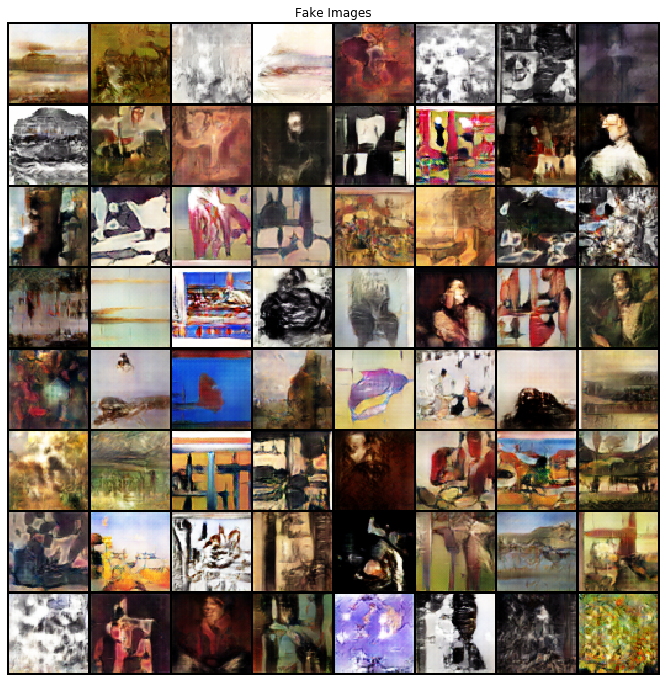
\includegraphics[width=0.7\linewidth]{../images/results/generated_data.png}
	\end{figure}
\end{frame}


%------------------------------------------------
\subsection{Resultados}
%------------------------------------------------

\begin{frame}
	\frametitle{Resultados}
	
\end{frame}

%------------------------------------------------
\subsection{Recursos y rendimiento}
%------------------------------------------------

\begin{frame}
	\frametitle{Recursos y rendimiento}
	
\end{frame}

%------------------------------------------------
\section{Arquitecturas basadas en GANs}
%------------------------------------------------

\begin{frame}
	\frametitle{Arquitecturas basadas en GANs}
	
\end{frame}

%------------------------------------------------
\section{Consideraciones pr�cticas}
%------------------------------------------------

\begin{frame}
	\frametitle{Consideraciones pr�cticas}
	
\end{frame}

%------------------------------------------------
\section{Conclusi�n}
%------------------------------------------------

\begin{frame}
\frametitle{Conclusi�n}

\end{frame}

%------------------------------------------------
\section{Referencias principales}
%------------------------------------------------

\begin{frame}
\frametitle{Referencias principales}
\begin{thebibliography}{9}


\end{thebibliography}
\end{frame}

%------------------------------------------------

\begin{frame}
\centering
\Huge
Gracias por su atenci�n. \par
\vfill
�Preguntas?
\end{frame}

\end{document}